% !TEX root = main.tex
%%%%%%%%%%%%%%%%%%%%%%%%%%%%%%%%%%%%%%%%%%%%%%%%%%%%%%%%%%%%%%%%%%%%%%%%%%%%%%%%
% Data Collection and Preprocessing
%%%%%%%%%%%%%%%%%%%%%%%%%%%%%%%%%%%%%%%%%%%%%%%%%%%%%%%%%%%%%%%%%%%%%%%%%%%%%%%%
\section{Data Collection and Preprocessing}
\label{section:dataprep}
Data on Titan GPU life times is constructed from two sources:
inventory runs and failure event records. Two types of failure events
were collected: Double Bit Error (DBE) and Off the Bus (OTB). Both
errors were found to be the ``signature'' event of GPU failures and a
trigger for their replacement.

An inventory of GPU serial numbers and their locations is recorded
each time the system boots. This typically occurs once every few days
but can be as frequent as a few times per day. A weekly inventory was
later added to run independently of system boots when they were fewer
and farther apart. A single inventory takes about a minute and is
recorded in a separate file. The DBE and OTB events are also recorded
separately from the inventories.  Figure~\ref{fig:inventory} shows
inter-inventory times that appear in the data.
\begin{figure}[bt]
  \begin{center}
    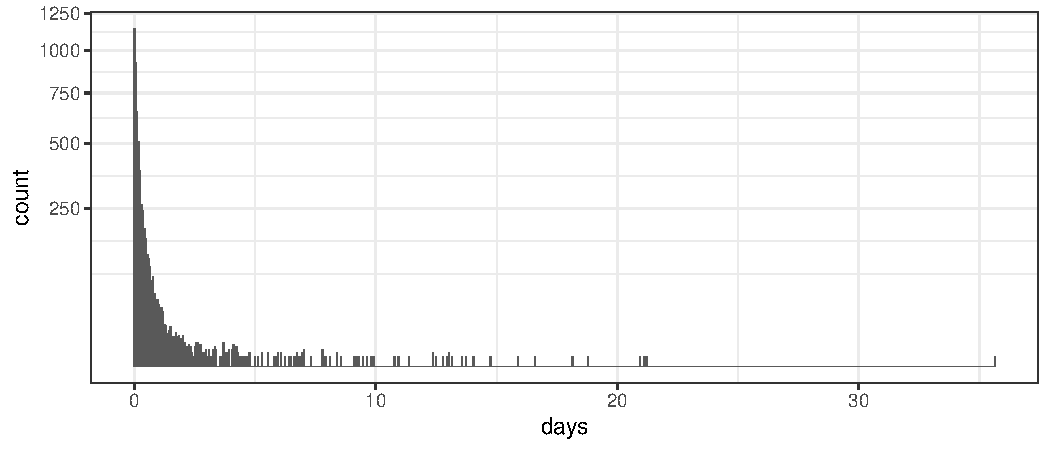
\includegraphics[width=\columnwidth]{figs/attention_intervals001.pdf}
  \end{center}
  \caption{Inter-inventory times, taken as time intervals between
    unique dates in the data and removing those less than a day. Note
    square root scale on the vertical axis.}
  \label{fig:inventory}
\end{figure}
Notably, there was a period of over a month and many periods of over a
week that Titan operated without a single reboot, especially in the
2014-2015 time frame.

Initial processing updates an inventory by checking the Serial Number
(SN) and Location of each GPU and creating or updating a separate
record for each contiguously observed SN-Location
combination. Resulting GPU data records are of the form shown in
Fig.~\ref{fig:dataraw},
\begin{figure}[tb]
{\tiny
\begin{verbatim}
0323812007945 | c17-4c1s3n1 | 01/10/2013 02:54:45 | 02/02/2013 11:32:29
 | c13-1c1s3n3 | 01/21/2014 21:10:42 | 08/01/2017 02:15:02
 | c0-1c1s3n3 | 10/11/2013 15:57:33 | 10/12/2013 22:09:31
 | c21-1c2s5n0 | 03/19/2013 15:48:11 | 05/29/2013 11:54:11
0325216047736 | c18-4c1s5n1 | 03/07/2017 02:15:01 | 03/12/2019 03:19:11
0323812008856 | c5-4c0s7n0 | 01/10/2013 02:54:45 | 01/25/2013 15:29:58
 | c0-6c1s7n2 | 10/21/2013 14:28:19 | 10/28/2013 17:52:44
 | c3-3c1s5n0 | 05/29/2013 11:54:11 | 05/29/2013 11:54:11
 | c23-6c1s7n2 | 01/21/2014 21:10:42 | 11/02/2018 14:42:34
 | | DBE | 11/02/2018 14:42:34
\end{verbatim}
}
\caption{A few records of raw data produced from inventories that is
  processed further in our analysis.}
\label{fig:dataraw}
\end{figure}
where records for three are shown. Each record starts
with a serial number and locations are coded with {\tt c{\it
    col-row}c{\it cage}s{\it slot}n{\it node}}. The location
references are cabinet column (0-24), row (0-7), cage (0-3), slot
(0-7), and node (0-3) with respect to the layout shown in
Figure~\ref{fig:layout}.
\begin{figure}
  \centering
  \begin{minipage}{0.49\columnwidth}
    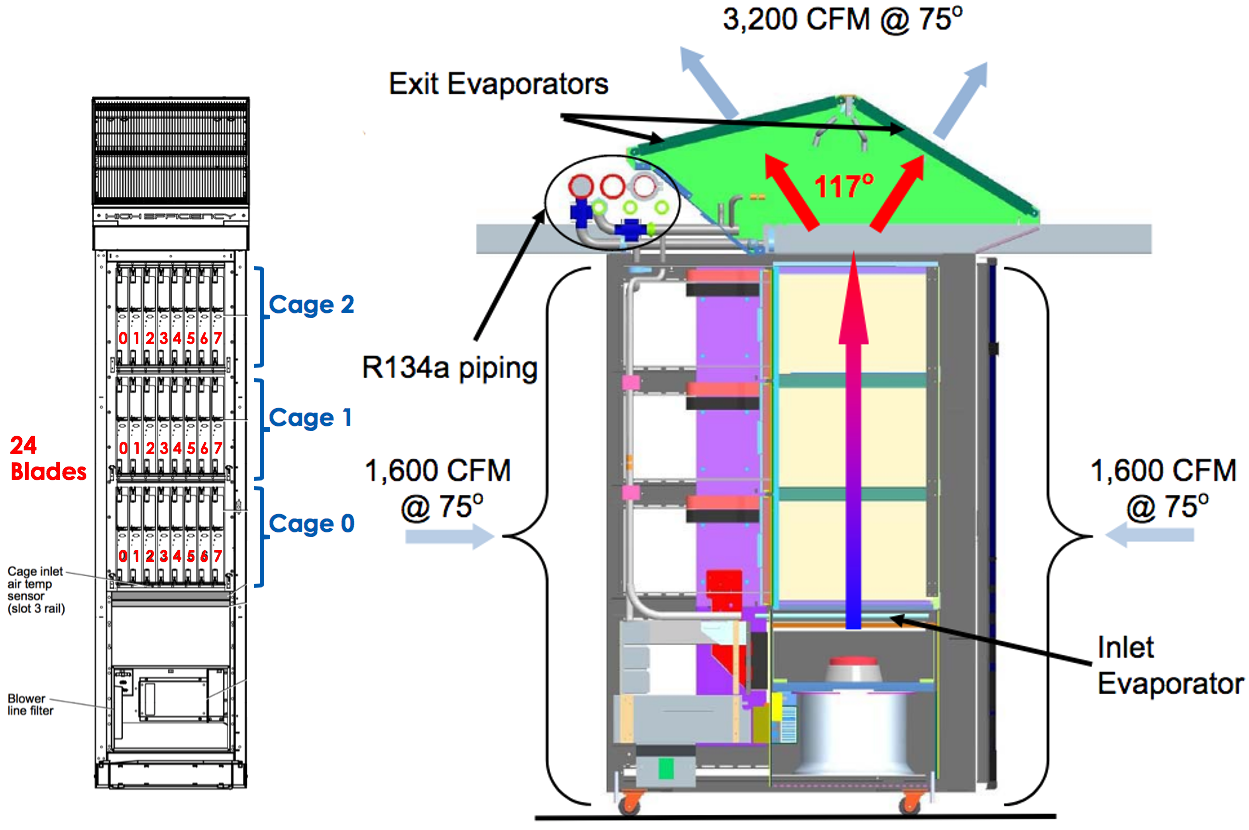
\includegraphics[width=\columnwidth]{figs/TitanCabinet.png}
    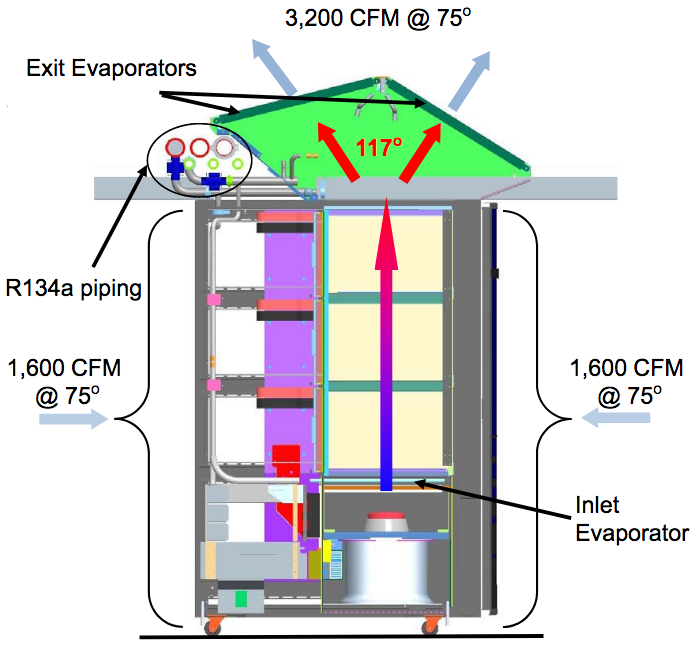
\includegraphics[width=0.9\columnwidth]{figs/TitanCabinetSide.png}
  \end{minipage}
  \begin{minipage}{0.49\columnwidth}
    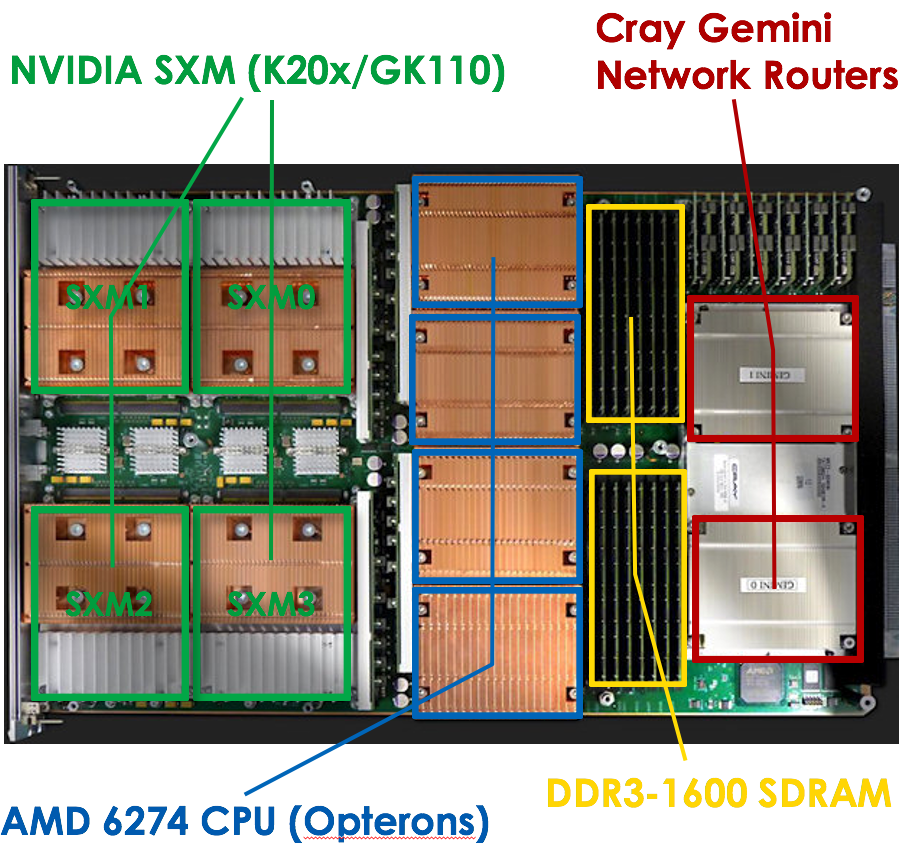
\includegraphics[width=\columnwidth]{figs/TitanBlade.png}

    \vspace{0.8\columnwidth}
    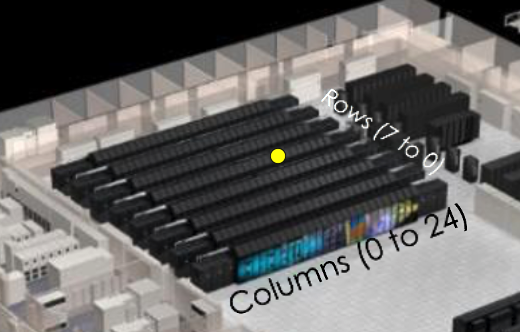
\includegraphics[width=\columnwidth]{figs/TitanLayout.png}
  \end{minipage}
  \caption{Titan cabinet (front view and side view with air flow) on
    the left, blade layout and floor layout on the right. Cooling
    airflow is bottom to top within a cabinet, taking ambient air in
    at the foot and relasing it back out at the top. Cooling fluid is
    passed through two heat exchange evaporators, one below Cage 0 and
    one above Cage 2.}
  \label{fig:layout}
\end{figure}


The first GPU record
shows installation in locations {\tt c17-4c1s3n1}, {\tt c21-1c2s5n0},
{\tt c0-1c1s3n3}, with periods off the system, and finally in {\tt
  c13-1c1s3n3}, where it stays until August 1, 2017, after which it is
not seen again. The second is installed in location {\tt c18-4c1s5n1},
where it stays until the last data collection date on March 3, 2019,
at 3:19:11 AM. The third GPU is first installed in locations {\tt
  c5-4c0s7n0}, {\tt c3-3c1s5n0}, {\tt c0-6c1s7n2}, and {\tt
  c23-6c1s7n2}, where a ``DBE'' is observed on November 2, 2018, and
it is not seen again.


% \fix{Where does cool air arrive? Is it just dumped out at the top of
%   the heat exchanger and circulate down? I noticed airholes in some
%   floor tiles (more on the right than on the left). Is there cool air
%   under the floor?}

% \fix{How does the coolant circulate? I notice three sets of pipes on
%   each side of each row: (2 x 3) x 8 = 48 sets.}
